% This is a basic Math Paper

\documentclass[11pt]{article}

% Preamble

\usepackage[margin=1in]{geometry}
\usepackage{amsfonts, amsmath, amssymb}
\usepackage{fancyhdr, float, graphicx}
\usepackage[utf8]{inputenc} % Required for inputting international characters
\usepackage[T1]{fontenc} % Output font encoding for international characters
\usepackage{fouriernc} % Use the New Century Schoolbook font
\usepackage[nottoc, notlot, notlof]{tocbibind}
\usepackage{url}

% Header and Footer
\pagestyle{fancy}
\fancyhead{}
\fancyfoot{}
\fancyhead[L]{\textit{\Large{Quantum Mechanics}}}
%\fancyhead[R]{\textit{something}}
\fancyfoot[C]{\thepage}
\renewcommand{\footrulewidth}{1pt}



% Other Doc Editing
% \parindent 0ex
%\renewcommand{\baselinestretch}{1.5}

\begin{document}
	
	\begin{titlepage} 
		\centering 
		
		%---------------------------NAMES-------------------------------
		
		\huge\textsc{
			MIT World Peace University
		}\\
	
		\vspace{0.75\baselineskip} % space after Uni Name
		
		\LARGE{
			Physics\\
			First Year B. Tech, Trimester 3\\
			Academic Year 2021-22
		}
		
		\vfill % space after Sub Name
		
		%--------------------------TITLE-------------------------------
		
		\rule{\textwidth}{1.6pt}\vspace*{-\baselineskip}\vspace*{2pt}
		\rule{\textwidth}{0.6pt}
		\vspace{0.75\baselineskip} % Whitespace above the title
		
		
		
		\huge{\textsc{
				Quantum Mechanics
			}} \\
		
		
		
		\vspace{0.5\baselineskip} % Whitespace below the title
		\rule{\textwidth}{0.6pt}\vspace*{-\baselineskip}\vspace*{2.8pt}
		\rule{\textwidth}{1.6pt}
		
		\vspace{1\baselineskip} % Whitespace after the title block

		%--------------------------SUBTITLE --------------------------	
			
		\LARGE\textsc{
			Notes
		} % Subtitle or further description
		\vfill
		
		%--------------------------AUTHOR-------------------------------
		
		Prepared By
		\vspace{0.5\baselineskip} % Whitespace before the editors
		
		\Large{
			109054. Krishnaraj Thadesar\\
			\vspace{1cm}
			Division 9 Batch I3
		}
		
		
		\vspace{0.5\baselineskip} % Whitespace below the editor list
		\today

	\end{titlepage}

\clearpage
\tableofcontents
\clearpage

\section{Brief History}

\subsection{Berlin 1890}
Germany is a new country, wanting to industrialize. Their engineers filed patents for the Edison Light bulb. Coz obviously they wanna make money from putting these bulbs in streets. \\

Now people knew that if you heat the filament, it glows, but people didnt know why. They didnt know why its yellow. How would you change the color and manufacture if you didnt know why? How would you increase the efficiency if you didnt know how it worked? So they made a new institute for stuff like this, and called upon a few noice scientists. One of them was Max Planck in 1900. \\

\textit{He took on a simple problem. Why does the color of light change if you increase its temperature? }\\

Planck made a blackbody identifier. They kept increasing the temperature, and realized that the temperature kept increasing, and the color kept changing as well.  But as they increased the temperature of the black body, they could get it to glow whiter and whiter, but they couldnt produce Ultravoilet light. The logic was simple, that more energy would produce light that had more energy. But even the sun wasn't producing a lot of Ultravoilet light. Why is that? \textit{This was named the ultravoilet catastrophe}\\

Around the same time, people were studying the Radio, which used Radio waves. In the process of experimentation was the Gold Leaf electroscope, which we built back in 7th grade. When you put charged things on it, the electrons in the gold leaf would repel, and so the gold leaves would repel. But they found that if you put ultravoilet light on this, the electrons are suddenly Knocked off. Electricity, and light these seemingly unrelated things, are now behaving like they know each other. Light can now remove static electricity! But only ultravoilet light can do that. \textit{This was the Photoelectric effect. }\\

Now, by this time, its widely accepted that Light is a wave. But this wave nature of light cant explain these 2 phenomena. \\

See, if light is a wave like you call it, then more intensity of the wave must mean more powerful waves isnt it? like if you go into the sea and notice how those huge waves will even knock ships off. This can happen coz more intense waves and more energy.... Right? So that should mean that more intense Red light should be able to knock off those electrons. But it doesnt. Why? Why do we need ultravoilet light? Weird isnt it? 

\subsection{Einstein 1905}

\textit{"No Reasonable definition of reality could be expected to permit Quantum Mechanics." - Einstein}\\

He was the first one who said, forget about light being a wave, maybe, its a particle? He used the words 'quantum' to describe the photon. He said that red light has very little frequency, and so it has less energy compared to ultravoilet. \\

\textit{Light was now a wave, and a particle...}\\

And it is for this discovery and explanation of the photoelectric effect that Einstein was awarded the Nobel Prize. It is also about the same time that he was inventing his theory of Relativity.\\

\subsection{The World 1922}

The Post War Era. Everything was changing. The rise and fall of world powers, the rise and fall of culture, revolutions, and people. In the midst of it all was the rise of Modern physics itself. Around this time the experiment that would shock the shit out of physicists was done in Bell Labs, New Jersey.\\

Just like we saw the interference pattern with light, they did an double slit experiment with electron beams, and noticed the same goddamn Pattern on the screen. This meant, the electrons have to be a wave. First light which was thought of as waves, starts behaving like particles, and now electrons which were thought of as particles, are starting to behave like waves? So the electrons were interfering with each other? \\

And it doesnt even end there. What if instead of a beam of electrons, you fired one electron at a time? then surely it wouldnt be able to interfere with other electrons right, coz they arent even there? Well it turns out you \textit{still} see the pattern. That basically means, that every single electron behaves like a wave. And this wave interferes with \textit{itself}, to contribute to the interference pattern. \\

\subsection{The Copenhagen Interpretation}
Neils Bohr, is the leader on this side of the war. He is a firm believer that the quantum world is vastly different from the real one, and bizarre as well. So bizarre, in fact, that when an electron is shot, it actually \textit{goes through both slits at the same time, and its wave then after passing through, it can actually simultaneously exist at all the points of the interference pattern, and only when we look at it, or make a detection, or place a screen is when you get to know where it actually is.} This is when your wave of probabilty collapses. This is known as the copenhagen interpretation, given copenhagen is the capital of Norway, and Neils Bohr was Dutch.  \\

Ofcourse, The other side of the war, was lead by Einstein. He hated this. He said that there is no way we dont know where the electron is unless we look at it. The moon doesnt just stop existing while I am not looking at it. These 2 men argued with each other for the next 10 years. \\

\subsection{Spooky Action at a distance}

Quantum entanglement is the physical phenomenon that occurs when a group of particles are generated, interact, or share spatial proximity in a way such that the quantum state of each particle of the group cannot be described independently of the state of the others, including when the particles are separated by a large distance. The topic of quantum entanglement is at the heart of the disparity between classical and quantum physics: entanglement is a primary feature of quantum mechanics lacking in classical mechanics.\\

Measurements of physical properties such as position, momentum, spin, and polarization performed on entangled particles can, in some cases, be found to be perfectly correlated.\\ And this is what Einstein didnt like. He said that this wasnt possible as it meant that these 2 entangled particles would be communicating faster than the speed of light. And that according to him wasn't possible. He said that the moment the particles are created, they are like a pair of gloves hidden in a box. Once you open the box, you realize whether or not you have the left or right one, the glove doesnt magically communicate with the other one. 
\begin{figure}
	\centering
	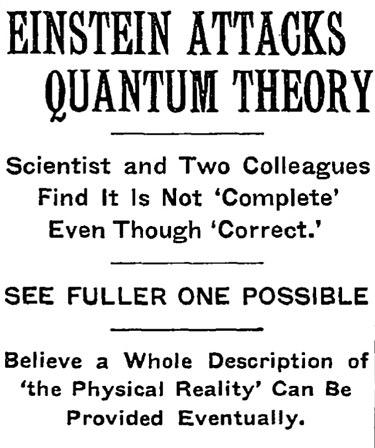
\includegraphics[scale=0.4]{newspaper.jpg}
	\caption{An article in the New York Times, May 4, 1935}
\end{figure}

\subsection{Development after the World War}
Soon after when the philosophical aspects of Quantum mechanics were highly debated, the world war broke out. And as it turned out, Believing Bohr's outlook, a lot of significant inventions, discoveries, and medical technology could be built. So people now didnt care about who was write. About the nature of reality itself, because the war was far more important. The Atomic Bomb is one such example. Einstein Died in 1955, still believing that 'God doesn't play dice'. And soon enough, a scientist in America, John Bell conducted experiments to see exactly who was right. Whether it was Einstein who believed that reality was like a pair of gloves, whose fate was destined at the time of creation and not measurement, or Bohr, who said the destiny of the entangled particle was decided upon measurement. \\

As it turns out, finally, Bohr was right after all. And the quantum world is as weird as it gets. But its beautiful. It can explain why enzymes can carry out reactions thousands of times faster than what would be physically possible, or how photosynthesis has such a staggering amount of efficiency, or how it may govern the laws of evolution itself. It also explains why Benzaldehyde and Cyanide smell the same. or why birds are able to migrate with unnatural sense of direction. \\

\textit{\textbf{Quantum theory is the most successful scientific theory of all time. Many of the great names of physics are associated with quantum theory. Heisenberg and Schrödinger established the mathematical form of the theory, while Einstein and Bohr analysed many of its important features. However, it was John Bell who investigated quantum theory in the greatest depth and established what the theory can tell us about the fundamental nature of the physical world.} }
\clearpage
\section{Phase Velocity and Group Velocity}

The phase velocity of a wave is the rate at which the particular phase of the wave propagates in space. 

\begin{equation}
	v_p = \frac{\omega}{k}
\end{equation}
So if you keep substituting a lot of equations that we have studied before, and we use the equation $y = A\sin(\omega t - kx)$, then you get the following
\begin{equation}
	v_p = \frac{c^2}{v} \implies v_p > c
\end{equation}
And that is not possible. So clearly we did something wrong. 
So in case of matter waves, what we do use is $y = A\sin(\omega t + d\omega - kxdx)$, and then you will get
\begin{equation}
	v_p = v_{particle} < c
\end{equation}
So what happens is that when a lot of these waves are travelling with each other, in case of matter, you get a group of particles superimposing, and interfering, and you will get nodes and anti nodes resulting in packets or envelops. 


\subsection{Properties of Matter waves}
\begin{enumerate}
	\item Matter particles are having wave nature. 
	\begin{equation}
		\lambda = \frac{h}{mv}
	\end{equation}	

	\item if m = constant, $\lambda$ is inversely proportional to v
	\item if v = constant, $\lambda$ is inversely proportional to m
	\item if v = 0, rest particle, they dont have wave nature. 
	\item Matter waves are not electromagnetic or mechanical in nature.
	\item Particle is localized in space, but waves are spread out, and you will have uncertainity in position of the particle. 
	\item $v_p = \frac{c^2}{v}$, Phase velocity of matter waves is greater than the light velocity.
	\item Wave particle nature cannot be exhibited simultainously. 
	\item These are called probability waves. 
	
\end{enumerate}

\subsection{Heisenberg's Uncertainity Principle }

It is impossible to determine both the exact position and exact momentum of the particle at the same time. 

\begin{eqnarray}
	\Delta x + m\Delta v =\frac{\hbar}{2}
\end{eqnarray}
use only h during numericals. 
\subsubsection{illustration of Uncertainity Principle using electron diffraction pattern from a single slit. }

\begin{equation}
	a \sin\theta = n\lambda
\end{equation}

This is a thought experiment. a was the slit width, and here we take that as $\Delta$y. And as usual the probability of the experiment landing on the screen can be predicted. You then apply the conservation of momentum. So then you would find the position, do some algebra, and would then arrive at the uncertainity principle. 


\section{Concept of Wave function and its physical significance}

$\Psi$ : The quantity which describes the de Broglie Wavelength. 
\begin{enumerate}
	\item The Probability of finding the particle in space (x, y, z), and hte time 't' is described by $\psi (x, y, z, t)$
	\item
	 \begin{eqnarray}
	 	\textit{Probability Density} = |\Psi \times dv|
%	 	\int_{-\infty}^{\infty} 	
	\end{eqnarray}
	
\end{enumerate}
\subsection{Schrodinger's Wave Equation}

He made Wave functions to describe the behavior of particle under the potential distribution. \\
Schrodinger: He supported the De-Broglie Hypothesis to develop the equations. 


\begin{eqnarray}
	\Psi(x, y, z, t) \textit{ has velocity u}\\
	\frac{\partial^2 \Psi}{\partial t^2} = u^2\Delta^2 \Psi\\
	\Delta^2 = \frac{\partial^2}{\partial x^2} + \frac{\partial^2}{\partial y^2} + \frac{\partial^2}{\partial z^2}\\
\end{eqnarray}

\subsection{Applications of Schrodinger's time independent wave equatins}

\begin{enumerate}
	\item 
	Schrodinger's wave equation: Behavior of particular in given space and time.
	\item To find the energy and the wave function of the system under given boundary conditions. 
	
	\item Particle in a Rigid Box (Infinity Potential Well): This is something like an electron inside an atom, where the atom is something like a well. The boundaries of the well have infinite potential, and so it becomes impossible for the electron to escape it. 

	\item Particle in non-rigid Box (Finite Potential Well)
	
	\item Tunneling Effect
\end{enumerate}



\end{document}